\documentclass[11pt]{article}

% Preamble

\usepackage[margin=1in]{geometry}
\usepackage{amsfonts, amsmath, amssymb}
\usepackage{fancyhdr, float, graphicx}
\usepackage[utf8]{inputenc} % Required for inputting international characters
\usepackage[T1]{fontenc} % Output font encoding for international characters
\usepackage{fouriernc} % Use the New Century Schoolbook font
\usepackage[nottoc, notlot, notlof]{tocbibind}
\usepackage{listings}
\usepackage{xcolor}

\definecolor{codegreen}{rgb}{0,0.6,0}
\definecolor{codegray}{rgb}{0.5,0.5,0.5}
\definecolor{codepurple}{rgb}{0.58,0,0.82}
\definecolor{backcolour}{rgb}{0.95,0.95,0.92}

\lstdefinestyle{mystyle}{
    backgroundcolor=\color{backcolour},   
    commentstyle=\color{codegreen},
    keywordstyle=\color{magenta},
    numberstyle=\tiny\color{codegray},
    stringstyle=\color{codepurple},
    basicstyle=\ttfamily\footnotesize,
    breakatwhitespace=false,         
    breaklines=true,                 
    captionpos=b,                    
    keepspaces=true,                 
    numbers=left,                    
    numbersep=5pt,                  
    showspaces=false,                
    showstringspaces=false,
    showtabs=false,                  
    tabsize=2
}

\lstset{style=mystyle}

% Header and Footer
\pagestyle{fancy}
\fancyhead{}
\fancyfoot{}
\fancyhead[L]{\textit{\Large{FDS Assignment 8}}}
%\fancyhead[R]{\textit{something}}
\fancyfoot[C]{\thepage}
\renewcommand{\footrulewidth}{1pt}

\begin{document}

\begin{titlepage}
	\centering

	%---------------------------NAMES-------------------------------

	\huge\textsc{
		MIT World Peace University
	}\\

	\vspace{0.75\baselineskip} % space after Uni Name

	\LARGE{
		Fundamental Data Structures\\
		Second Year B. Tech, Semester 1
	}

	\vfill % space after Sub Name

	%--------------------------TITLE-------------------------------

	\rule{\textwidth}{1.6pt}\vspace*{-\baselineskip}\vspace*{2pt}
	\rule{\textwidth}{0.6pt}
	\vspace{0.75\baselineskip} % Whitespace above the title

	\huge{\textsc{
			Expression Evaluation using stack
		}} \\



	\vspace{0.5\baselineskip} % Whitespace below the title
	\rule{\textwidth}{0.6pt}\vspace*{-\baselineskip}\vspace*{2.8pt}
	\rule{\textwidth}{1.6pt}

	\vspace{1\baselineskip} % Whitespace after the title block

	%--------------------------SUBTITLE --------------------------	

	\LARGE\textsc{
		Practical Report\\
		Assignment 8
	} % Subtitle or further description
	\vfill

	%--------------------------AUTHOR-------------------------------

	Prepared By
	\vspace{0.5\baselineskip} % Whitespace before the editors

	\Large{
		Krishnaraj Thadesar \\
		Cyber Security and Forensics\\
		Batch A1, PA 20
	}


	\vspace{0.5\baselineskip} % Whitespace below the editor list
	\today

\end{titlepage}


\tableofcontents
\thispagestyle{empty}
\clearpage
\setcounter{page}{1}

\section{Aim}
Writing a C Program to Evaluate a Postfix Expression using Stack.
\section{Objectives}
\begin{enumerate}
	\item To study Stack and its operations
	\item To study the importance of expression evaluation
\end{enumerate}

\section{Problem Statements}
\textit{Write a C Program to Evaluate a Postfix Expression using Stack. }

\section{Theory}
\textbf{Example of Working of Evaluation: 2 10 + 9 6 - /}\\
\begin{enumerate}
	\item First push 2 and 10 on the stack\\
	      \begin{figure}[H]
		      \centering
		      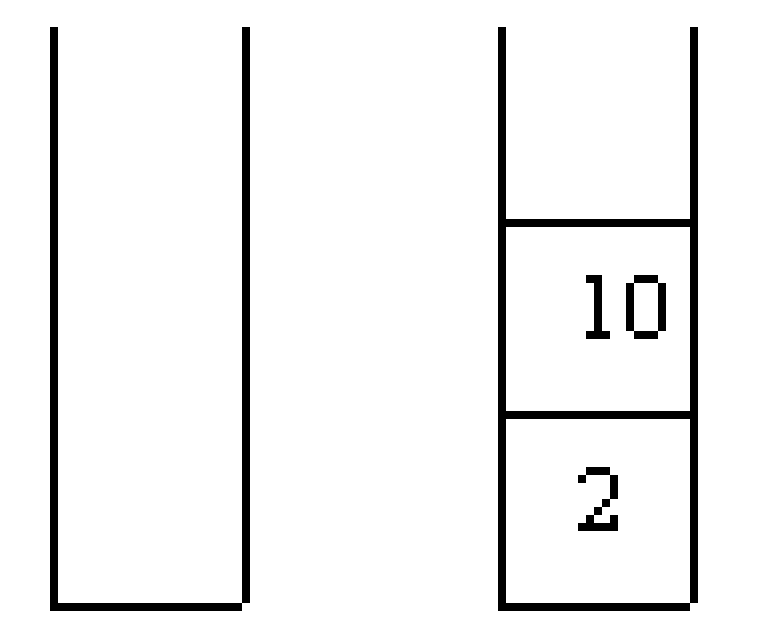
\includegraphics[width=0.25\textwidth]{stack 1.png}
		      \caption{After 2 and 10 are pushed}
	      \end{figure}
	\item Calculate 2 + 10 and then push 12 on the stack\\

	      \begin{figure}[H]
		      \centering
		      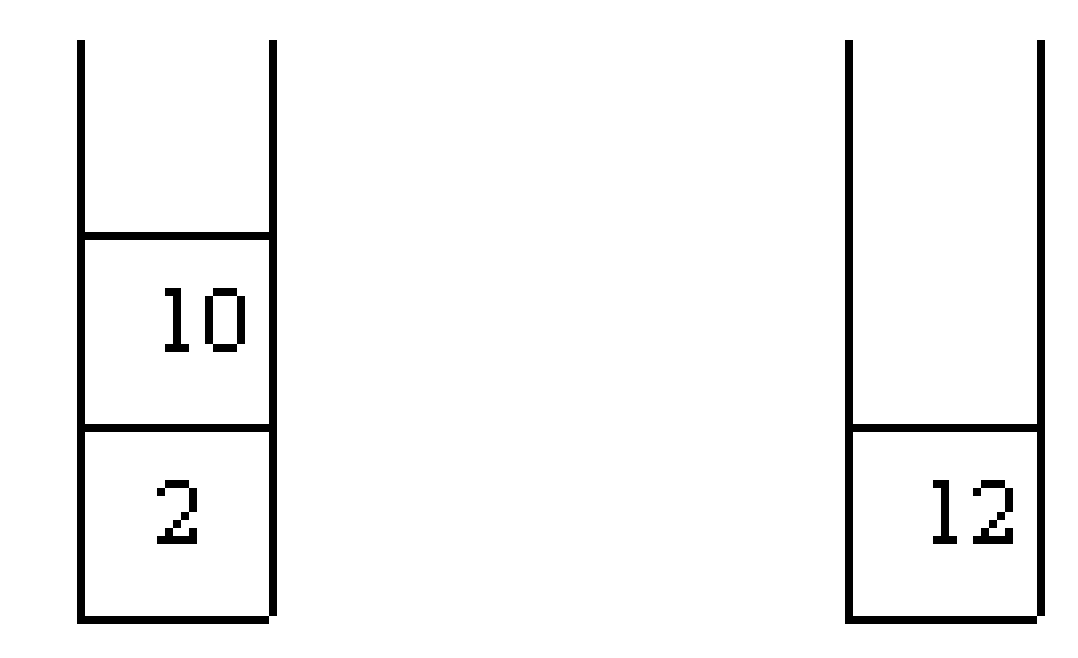
\includegraphics[width=0.25\textwidth]{stack 2.png}
		      \caption{After 12 is pushed}
	      \end{figure}
	\item Then push 6 and 9 on the stack\\

	      \begin{figure}[H]
		      \centering
		      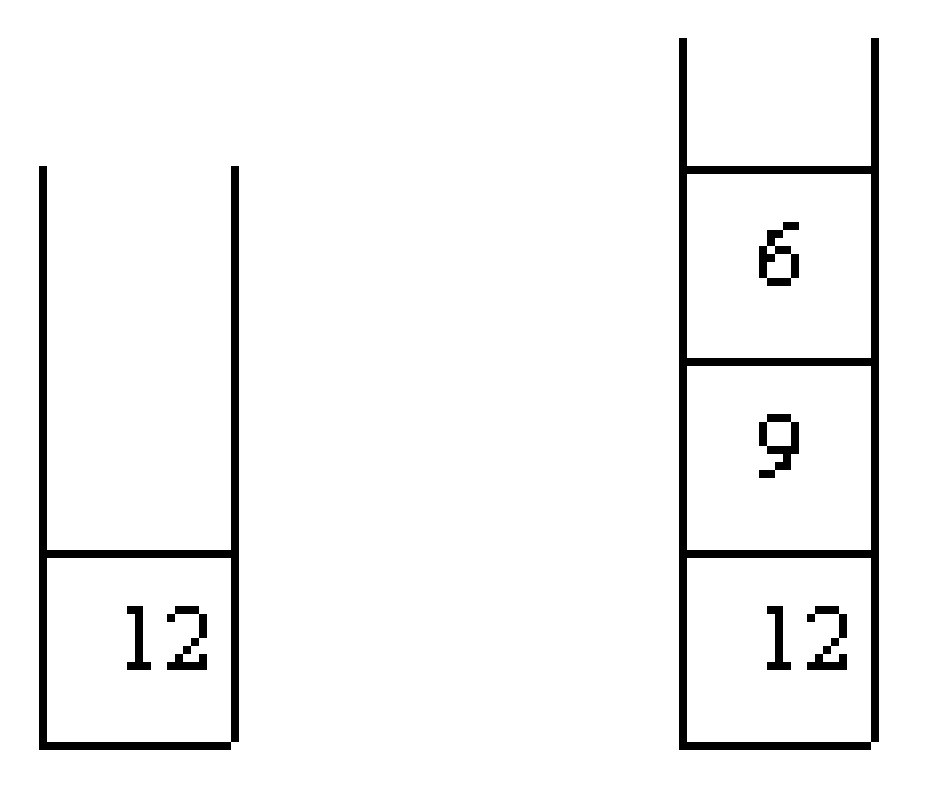
\includegraphics[width=0.25\textwidth]{stack 3.png}
		      \caption{After 6 and 9 are pushed}
	      \end{figure}
	\item Then Calculate 9 - 6 and push 3 on the stack\\

	      \begin{figure}[H]
		      \centering
		      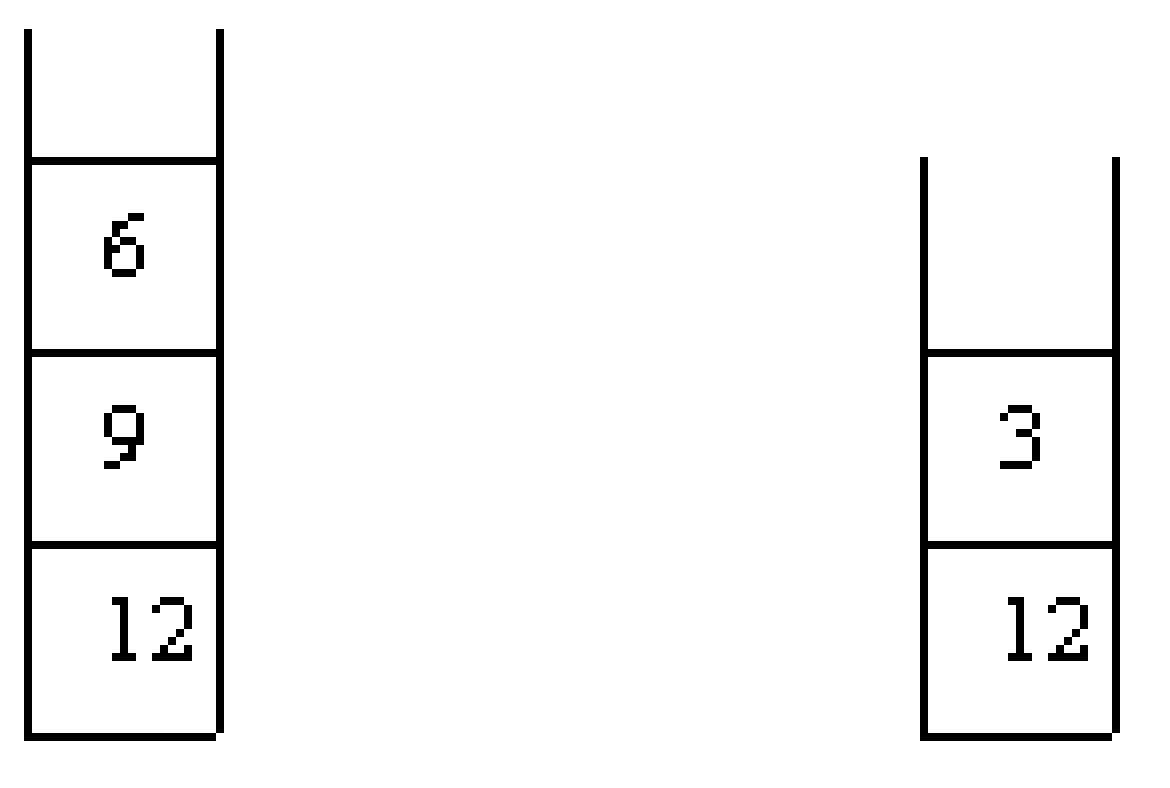
\includegraphics[width=0.25\textwidth]{stack 4.png}
		      \caption{After 3 and 12 are pushed}
	      \end{figure}
	\item Finally Calculate 12 / 3 and push 4 on the stack\\

	      \begin{figure}[H]
		      \centering
		      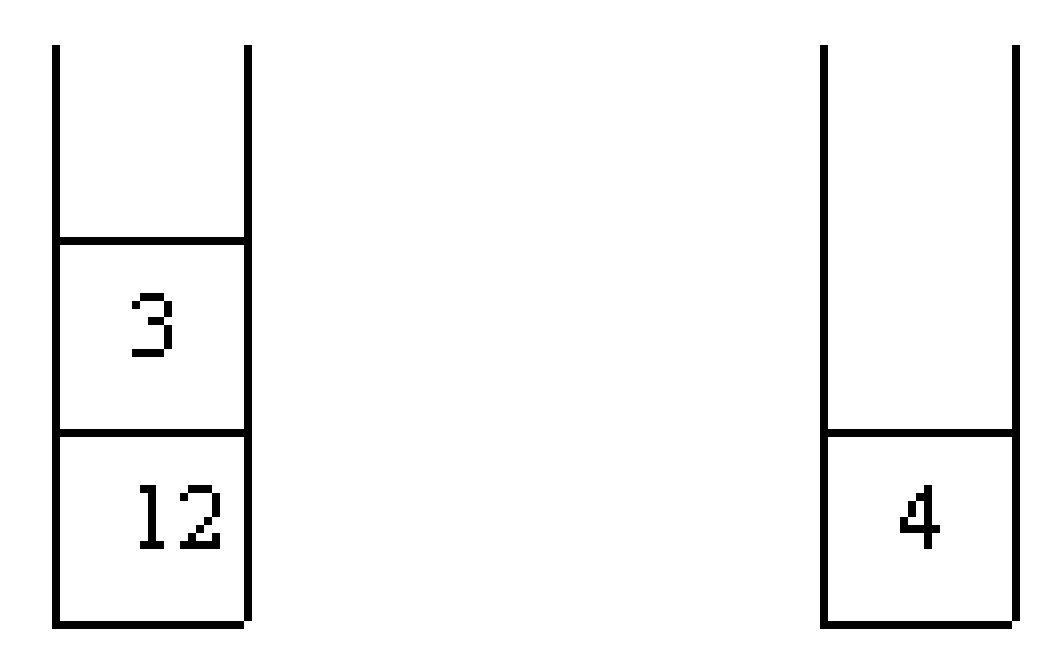
\includegraphics[width=0.25\textwidth]{stack 5.png}
		      \caption{After result is pushed}
	      \end{figure}
\end{enumerate}
\section{Platform}
\textbf{Operating System}: Arch Linux x86-64 \\
\textbf{IDEs or Text Editors Used}: Visual Studio Code\\
\textbf{Compilers} : gcc on linux for C\\

\section{Input}
The Postfix Condition
\section{Output}
The Evaluation of the Postfix Expression entered.
\section{Test Conditions}
The Postfix Expression and Checking its Evaluation.
\section{Code}
\subsection{Pseudo Code for calc}
\begin{lstlisting}[language=C]
	calc(op1, op2, op)
		ans;
		switch (op)
			case '+':
				ans = op1 + op2;
				break;
			case '-':
				ans = op1 - op2;
				break;
			case '*':
				ans = op1 * op2;
				break;
			case '/':
				ans = op1 / op2;
				break;
			case '%':
				ans = op1 % op2;
				break;
			case '^':
				ans = powerr(op1, op2);
				break;
			default:
				printf("\nInvalid operator");
				break;
		return ans;
\end{lstlisting}
\subsubsection{Pseudo Code for Eval}

\begin{lstlisting}[language=C]
	eval(char post[MAX_SIZE])
		int z = 0, ans = 0, op1, op2;
		for (int i = 0; post[i] != 0; i++)
			if(ISALPHA(post[i]))
				print("\nEnter value of %c: ", post[i]);
				scan("%d", &z);
				push(z);
			else
				op1 = pop();
				op2 = pop();
				ans = calc(op2, op1, post[i]);
				push(ans);
		print("\nAnswer = %d\n", stack[top]);
\end{lstlisting}
\subsection{C Implementation of Problem Statement}

\lstinputlisting[language=C, caption=Main.Cpp]{../Programs/[Krishnaraj]_[FDS]_Assignment_8.c}

\subsection{Input and Output}
\lstinputlisting[caption=Output]{../Programs/[Krishnaraj]_[FDS]_Assignment_8_output.txt}

\section{Time Complexity}
\begin{itemize}
	\item clac() : O(n)
	\item eval() : O(n) where n is the length of the post array.
\end{itemize}

\section{Conclusion}
Thus, implemented postfix expression evaluation using stack data structure.


\section{FAQs}
\begin{enumerate}
	\item \textbf{How does prefix expression evaluation work?}\\
	      In this notation, operator is prefixed to operands, i.e. operator is written ahead of operands. For example, +ab. This is equivalent to its infix notation a + b. Prefix notation is also known as Polish Notation.

	      \begin{enumerate}
		      \item Step 1: Start from the last element of the expression.

		      \item Step 2: check the current element.

		      \item Step 2.1: if it is an operand, push it to the stack.
		      \item Step 2.2: If it is an operator, pop two operands from the stack. Perform the operation and push the elements back to the stack.

		      \item Step 3: Do this till all the elements of the expression are traversed and return the top of stack which will be the result of the operation.
	      \end{enumerate}
	\item \textbf{What is the advantage of prefix and postfix expressions?}\\

	      \begin{enumerate}
		      \item Prefix notations are needed when we require operators before the operands while postfix notations are needed when we require operators after the operands.
		      \item Prefix notations are used in many programming languages like LISP.
		      \item Prefix notations and Prefix notations can be evaluated faster than the infix notation.
		      \item Postfix notations can be used in intermediate code generation in compiler design.
		      \item Prefix and Postfix notations are easier to parse for a machine.
		      \item With prefix and postfix notation there is never any question like operator precedence.
		      \item There is no issue of left-right associativity.
	      \end{enumerate}

\end{enumerate}
\end{document}

